%Version 2.1 April 2023
% See section 11 of the User Manual for version history
%
%%%%%%%%%%%%%%%%%%%%%%%%%%%%%%%%%%%%%%%%%%%%%%%%%%%%%%%%%%%%%%%%%%%%%%
%%                                                                 %%
%% Please do not use \input{...} to include other tex files.       %%
%% Submit your LaTeX manuscript as one .tex document.              %%
%%                                                                 %%
%% All additional figures and files should be attached             %%
%% separately and not embedded in the \TeX\ document itself.       %%
%%                                                                 %%
%%%%%%%%%%%%%%%%%%%%%%%%%%%%%%%%%%%%%%%%%%%%%%%%%%%%%%%%%%%%%%%%%%%%%

\documentclass[sn-basic,Numbered,iicol,pdflatex]{sn-jnl}

%%%% Standard Packages
%%<additional latex packages if required can be included here>

\usepackage{graphicx}%
\usepackage{multirow}%
\usepackage{amsmath,amssymb,amsfonts}%
\usepackage{amsthm}%
\usepackage{mathrsfs}%
\usepackage[title]{appendix}%
\usepackage{xcolor}%
\usepackage{textcomp}%
\usepackage{manyfoot}%
\usepackage{booktabs}%
\usepackage{algorithm}%
\usepackage{algorithmicx}%
\usepackage{algpseudocode}%
\usepackage{listings}%
\usepackage{orcidlink}%
%%%%

%%%%%=============================================================================%%%%
%%%%  Remarks: This template is provided to aid authors with the preparation
%%%%  of original research articles intended for submission to journals published
%%%%  by Springer Nature. The guidance has been prepared in partnership with
%%%%  production teams to conform to Springer Nature technical requirements.
%%%%  Editorial and presentation requirements differ among journal portfolios and
%%%%  research disciplines. You may find sections in this template are irrelevant
%%%%  to your work and are empowered to omit any such section if allowed by the
%%%%  journal you intend to submit to. The submission guidelines and policies
%%%%  of the journal take precedence. A detailed User Manual is available in the
%%%%  template package for technical guidance.
%%%%%=============================================================================%%%%




\raggedbottom

\unnumbered



% tightlist command for lists without linebreak
\providecommand{\tightlist}{%
  \setlength{\itemsep}{0pt}\setlength{\parskip}{0pt}}

% From pandoc table feature
\usepackage{longtable,booktabs,array}
\usepackage{calc} % for calculating minipage widths
% Correct order of tables after \paragraph or \subparagraph
\usepackage{etoolbox}
\makeatletter
\patchcmd\longtable{\par}{\if@noskipsec\mbox{}\fi\par}{}{}
\makeatother
% Allow footnotes in longtable head/foot
\IfFileExists{footnotehyper.sty}{\usepackage{footnotehyper}}{\usepackage{footnote}}
\makesavenoteenv{longtable}




\begin{document}


\title[]{Substitution of red meat with legumes and risk of primary liver cancer in 126,744 UK Biobank participants: a prospective cohort study}

%%=============================================================%%
%% Prefix	-> \pfx{Dr}
%% GivenName	-> \fnm{Joergen W.}
%% Particle	-> \spfx{van der} -> surname prefix
%% FamilyName	-> \sur{Ploeg}
%% Suffix	-> \sfx{IV}
%% NatureName	-> \tanm{Poet Laureate} -> Title after name
%% Degrees	-> \dgr{MSc, PhD}
%% \author*[1,2]{\pfx{Dr} \fnm{Joergen W.} \spfx{van der} \sur{Ploeg} \sfx{IV} \tanm{Poet Laureate}
%%                 \dgr{MSc, PhD}}\email{iauthor@gmail.com}
%%=============================================================%%

\author[1]{\fnm{Niels} \sur{Bock} \orcidlink{0009-0005-7373-1589}}

\author[1]{\fnm{Fie} \sur{Langmann} \orcidlink{0000-0003-3474-9346}}

\author[1,2]{\fnm{Luke} \spfx{W.} \sur{Johnston} \orcidlink{0000-0003-4169-2616}}

\author[1,2,3,4]{\fnm{Daniel} \spfx{B.} \sur{Ibsen} \orcidlink{0000-0002-7038-4770}}

\author*[1]{\fnm{Christina} \spfx{C.} \sur{Dahm} \orcidlink{0000-0003-0481-2893}}\email{\href{mailto:ccd@ph.au.dk}{\nolinkurl{ccd@ph.au.dk}}}



  \affil*[1]{\orgdiv{Department of Public Health}, \orgname{Aarhus University}, \orgaddress{\city{Aarhus}, \country{Denmark}}}
  \affil[2]{\orgdiv{Steno Diabetes Center}, \orgname{Aarhus University}, \orgaddress{\city{Aarhus}, \country{Denmark}}}
  \affil[3]{\orgdiv{Department of Nutrition, Exercise and Sports}, \orgname{University of Copenhagen}, \orgaddress{\city{Copenhagen}, \country{Denmark}}}
  \affil[4]{\orgdiv{MRC Epidemiology Unit, School of Clinical Medicine}, \orgname{University of Cambridge}, \orgaddress{\city{Cambridge}, \country{United Kingdom}}}

\abstract{\textbf{Purpose}: Primary liver cancer is on the rise worldwide, partially due to poor diets and sedentary lifestyles. Shifting to more plant-based diets may lower the risk. We aimed to estimate the effect of replacing unprocessed red meat, processed red meat and total red meat with legumes on primary liver cancer in a free-living population.

\textbf{Methods}: We analyzed data from 126,744 UK Biobank participants who completed \(\geq\) 2 24-hour diet recall questionnaires. Baseline characteristics were collected from the initial assessment visit. Information on liver cancer diagnoses was collected via external linkage to inpatient hospital episodes or central cancer registries. Cox proportional hazards regression models were used to estimate substitution of 15g/day of legumes with 15/day of total red meat, unprocessed red meat and processed red meat on liver cancer risk, using the leave-one-out food substitution model.

\textbf{Results}: During a median follow-up time of 11.3 years, 173 participants developed liver cancer. In the fully adjusted models, no association was observed when substituting 15/day of legumes with total red meat (HR: 0.98 (95\% CI 0.93-1.04)), unprocessed red meat (HR: 0.97 (95\% CI 0.91-1.03)) or processed red meat (HR: 1.02 (95\% CI 0.93-1.13)).

\textbf{Conclusion}: Overall, little evidence of an association between replacing red meat with legumes and liver cancer was observed. Further research in larger study populations with longer follow-up time is warranted.}

\keywords{Food Substitutions, Liver cancer, Red meat, Legumes}



\maketitle

\clearpage

\hypertarget{sec1}{%
\section{Background}\label{sec1}}

Hepatocellular carcinoma (HCC) is the sixth most common cancer in the
world and the third leading cause of cancer-related death with viral
hepatitis being the main risk factor {[}1-3{]}. However, in Western
countries, the increase of non-alcoholic fatty liver disease (NAFLD),
the most common chronic liver disease worldwide {[}4, 5{]}, has become a
major risk factor for liver cancer {[}3, 6, 7{]}. NAFLD is mainly caused by
a sedentary lifestyle and a diet high in fats and red meats and
concurrently low in fruit, vegetables, and whole grains {[}5{]} and could be
considered as the hepatic manifestation of metabolic syndrome {[}8{]}. The
prevalence of NAFLD-related HCC cases is an increasing global problem
{[}7{]}, and it is estimated that prevalent cases of NAFLD-related HCC in
the US will increase by 146\%, from 10,100 to 24,900 cases, while
incident NAFLD-related HCC cases will increase by 137\%, from 5,160 to
12,240 cases, in 2030 {[}9{]}.

The second most common primary liver cancer is the intrahepatic
cholangiocarcinoma (ICC) {[}10{]}. While HCC emerges from the liver
parenchyma, ICC emerges from the bile duct. Despite being a relatively
rare cancer, ICC is characterized by its aggressivity, late diagnosis
and poor survival {[}11{]}. It is estimated that the incidence of ICC is on
the rise worldwide {[}12, 13{]}. Three recent meta-analyses have established
evidence of an adverse association between NAFLD and ICC {[}14-16{]}.

Consumption of legumes may protect against type 2 diabetes due to better
glycemic control and reduced risk of metabolic syndrome {[}20, 22, 23{]}.
Legumes have hypolipidemic and hypotensive effects, which have been
proposed as the cause of the inverse association between legume
consumption and cardiovascular disease. {[}24-27{]} They further contain
phytochemicals such as bioactive peptides, polyphenols, and other
antioxidants with anticarcinogenic properties {[}28-30{]}. Several
epidemiological studies have investigated the effect of soy and non-soy
legume consumption on different cancers with promising results {[}31, 32{]}.
Legume consumption has been linked to a reduced risk of colorectal
adenoma and colorectal cancer {[}33, 34{]}, prostate cancer {[}35, 36{]}, renal
cell carcinoma {[}37, 38{]}, and endometrial cancer {[}39{]}.

Studies on diet and liver cancer suggest that increased vegetable intake
is inversely associated with liver cancer {[}40-43{]}. Two large prospective
cohort studies found inverse associations between legume consumption and
risk of HCC {[}40, 42{]}. However, replacement foods were not specified in
these studies, and thus the association between eating more legumes and
concomitantly less meat is unclear.

Studies on substituting plant protein for animal protein are important
as we need to eat less animal-based foods and more plants to lower the
climate impact of our diet {[}47{]}. Although previous research has
investigated substitution of animal-based proteins with plant-based
proteins in relations to NAFLD {[}48{]}, research on substituting meats with
legumes in relation to risk of HCC and IH-CCA is sparse. This leaves a
substantial gap in our current knowledge on the beneficial effects on
primary liver cancer from substituting meats with legumes.

The main aim of this study was to estimate the effect of replacing
unprocessed red meat, processed red meat and total red meat with legumes
on primary liver cancer in a free-living population.

\hypertarget{sec2}{%
\section{Research Design and Methods}\label{sec2}}

\hypertarget{subsec1}{%
\subsection{Study population}\label{subsec1}}

The UK Biobank, a population-based prospective cohort, was initiated in
2006. \citep{sudlow2015} During 2006-2010, more than 500,000 participants,
aged 40-69, were recruited and visited designated assessment centres
across the UK Participants provided information about age, sex,
sociodemographic factors (education, Townsend deprivation index, living
alone) and lifestyle factors (smoking, alcohol consumption, physical
activity) via touch screen questionnaires and computer-assisted
interviews. Anthropometric data (waist circumference) were collected via
physical measurements \citep{RN113}.

\hypertarget{subsec2}{%
\subsection{Dietary assessment}\label{subsec2}}

A web-based 24-hour dietary recall was administered at the end of the
initial assessment visit for the last 70,000 recruited participants
\citep{RN115}. From February 2011 to April 2012, 320,000 participants who had
provided an e-mail address were invited on four separate occasions to
complete the 24-hour dietary recall, the Oxford WebQ, of which 210,947
participants completed at least one. The Oxford WebQ covered 206 food
items and 32 beverage items commonly consumed in the UK. Intakes were
reported in standard units of measurements, e.g., servings, cups,
slices, etc. with intake categories ranging from 0 to 3+ units
\citep{piernas2021}. The Oxford WebQ has been validated against
interviewer-based 24-hour dietary recalls and biomarkers \citep{Liu2011, Greenwood2019}.

Researchers defined 79 food groups and 14 beverage groups from the
Oxford WebQ using the UK National Diet and Nutrition Survey categories
\citep{piernas2021}. These food and beverage groups were used when defining
the food groups used in the substitution analyses (Supplementary Table
1). Legumes were defined as dietary pulses, baked beans, tofu-based
products, peas, hummus, soy drinks, and soy-based desserts and yogurt.
Red meat intake was defined as intake of beef, pork, lamb, or other
meat, including offal. Processed red meat intake was defined as
sausages, bacon (with and without fat), ham, or liver pate. Other food
groups included were animal-based foods, unhealthy plant-based foods,
healthy plant-based foods, and alcoholic beverages (Supplementary Table
1). Animal-based and healthy and unhealthy plant-based food foods were
grouped based on plant-based diet indices from previous studies
\citep{Thompson2023, Heianza2021, Satija2017, Satija2016}. An overview of
included foods in each food group is displayed in Table
\ref{tab-food-group}.

As a single 24-hour dietary recall does not assess habitual dietary
intake and variation in diet over time at an individual level
\citep{thompson2013, gurinovic2017}, only participants who completed two or
more Oxford WebQs were eligible for inclusion in this study.

\hypertarget{subsec3}{%
\subsection{Liver cancer assessment}\label{subsec3}}

Liver cancer was defined according to ICD-10 diagnosis codes C22.0 for
Hepatocellular carcinoma (HCC) or C22.1 for Intrahepatic
cholangiocarcinoma (ICC) and ICD-9 diagnosis codes 1550 Malignant
neoplasm of liver, primary or 1551 Malignant neoplasm of intrahepatic
bile ducts. Incident and prevalent cases of liver cancer and
corresponding diagnosis dates were obtained via external linkage to
central cancer registries or hospital inpatient episodes \citep{RN112, RN114}.

\hypertarget{subsec4}{%
\subsection{Assessment of confounders}\label{subsec4}}

Confounders were defined \emph{a priori} from a literature review of the
background literature and illustrated using directed acyclic graphs
(Figure \ref{fig:fig2}). The following confounding variables were
selected: age at baseline (years, continuous), sex (male, female),
educational level (high: College or University degree, intermediate: A
levels/AS levels, O levels/GCSEs, or equivalent, low: none of the
previous mentioned), Townsend Deprivation Index (continuous), Living
alone (yes, no), waist circumference (cm, continuous), physical activity
(above/below the 2017 UK Physical activity guidelines of 150 minutes of
moderate activity per week or 75 minutes of vigorous activity, or
unknown), smoking (pack years as a proportion of lifespan exposed to
smoking, continous), and alcohol intake (g/day, continuous). All
confounders except age were selected from the initial assessment visit
before the start of follow-up.

\hypertarget{subsec5}{%
\subsection{The substitution model}\label{subsec5}}

The substitution analyses were conducted by by modelling replacement of
an equal mass of meat with legumes. The portion size of the substitution
was set to 15 g of legumes for 15 g of meat to ensure that substitutions
were below the mean intake of any of the substituted food groups in the
cohort. The substitutions were modeled using the leave-one-out-approach
in which variables for every food group along with a variable for total
food intake are included, except the food group that are to be
substituted \citep{Ibsen2021}. To estimate substitution of 15 g of all red
meats (red and processed) with 15 g of legumes, the following model was
defined:

\begin{align}
\log(h(t;x)) &= \log(h_0(t)) \nonumber \\
&\quad + \beta_1 \text{Legumes (15g)} \nonumber \\
&\quad + \beta_2 \text{Total food intake (g)} \nonumber \\
&\quad + \beta_3 \text{Other food groups (g)} \nonumber \\
&\quad + \beta_4 \text{Covariates}
\end{align}

\noindent When substituting only red meat with legumes, processed red
meat was added to the model:

\begin{align}
\log(h(t;x)) &= \log(h_0(t)) \nonumber \\
&\quad + \beta_1 \text{Legumes (15g)} \nonumber \\
&\quad + \beta_2 \text{Processed red meat (15g)} \nonumber \\
&\quad + \beta_3 \text{Total food intake (g)} \nonumber \\
&\quad + \beta_4 \text{Other food groups (g)} \nonumber \\
&\quad + \beta_5 \text{Covariates}
\end{align}

\noindent When substituting only processed red meat with legumes, red
meat was added to the model:

\begin{align}
\log(h(t;x)) &= \log(h_0(t)) \nonumber \\
&\quad + \beta_1 \text{Legumes (15g)} \nonumber \\
&\quad + \beta_2 \text{Red meat (15g)} \nonumber \\
&\quad + \beta_3 \text{Total food intake (g)} \nonumber \\ 
&\quad + \beta_4 \text{Other food groups (g)} \nonumber \\
&\quad + \beta_5 \text{Covariates}
\end{align}

\noindent The performance of the leave-one-out model when modeling equal
mass substitutions has been validated against simulated data
\citep{Tomova2022}.

\hypertarget{subsec6}{%
\subsection{Statistical analysis}\label{subsec6}}

Multivariable-adjusted Cox proportional hazards regression models were
used to estimate hazard ratios (HR) with corresponding 95\% confidence
intervals (CI) with age as the underlying timescale. Participants were
followed from the date of their last completed Oxford WebQ until the
occurrence of the event of interest or due to right censoring, whichever
came first. Participants were right censored in the event of death, loss
to follow-up, or administrative end of follow-up (October 31, 2022). Two
levels of adjustments were added to the substitution model. Model 1 was
minimally adjusted for age, total weight of food intake, and all other
food groups to fit the substitution model. Model 2 was further adjusted
for sex, educational level, Townsend Deprivation Index, living alone,
physical activity, smoking, alcohol intake, and waist circumference.

In secondary analyses, each cancer type was analysed separately to
evaluate if the pooling of HCC and ICC as one outcome in the main
analysis was justified. Furthermore, to estimate the association of
legume intake with liver cancer regardless of other dietary components,
legume consumers (divided into quartiles) were compared to
non-consumers.

To evaluate the robustness of the main analyses, sensitivity analyses
were performed on subsamples of participants by excluding those with
high alcohol intake (exclusion of upper decile of daily alcohol intake
by sex), implausible energy intake (exclusion of upper and lower deciel
of each sex), any liver disease before baseline, any type of cancer
before baseline, and fewer than 3 completed Oxford WebQs. As neither the
central cancer registries nor the hospital inpatient registries were
complete, liver cancer diagnoses retrieved from death registries, which
were more up-to-date, were included in a sensitivity analysis to test
for outcome misclassification bias. Lastly, one of our causal
assumptions was that anthropometry confounded the causal relationship
between replacing red meat with legumes and liver cancer; however,
strong arguments exist giving support to anthropometry being a mediator
between diet and health outcomes. Thus, to test for erroneously
conditioning on a potential mediator, waist circumference was removed in
a sensitivity analysis. Sensitivity analyses were modeled as the fully
adjusted models in the main analyses.

All analyses were conducted in R (version 4.1.1) with a significance
level of 5 \%.

\hypertarget{sec3}{%
\section{Results}\label{sec3}}

After excluding participants with liver cancer before baseline,
participants lost to follow-up before baseline, and participants with
errors in dietary data, 126,744 participants who had completed two or
more diet questionnaires remained (Figure \ref{fig:fig1}).

\begin{figure*}

{\centering 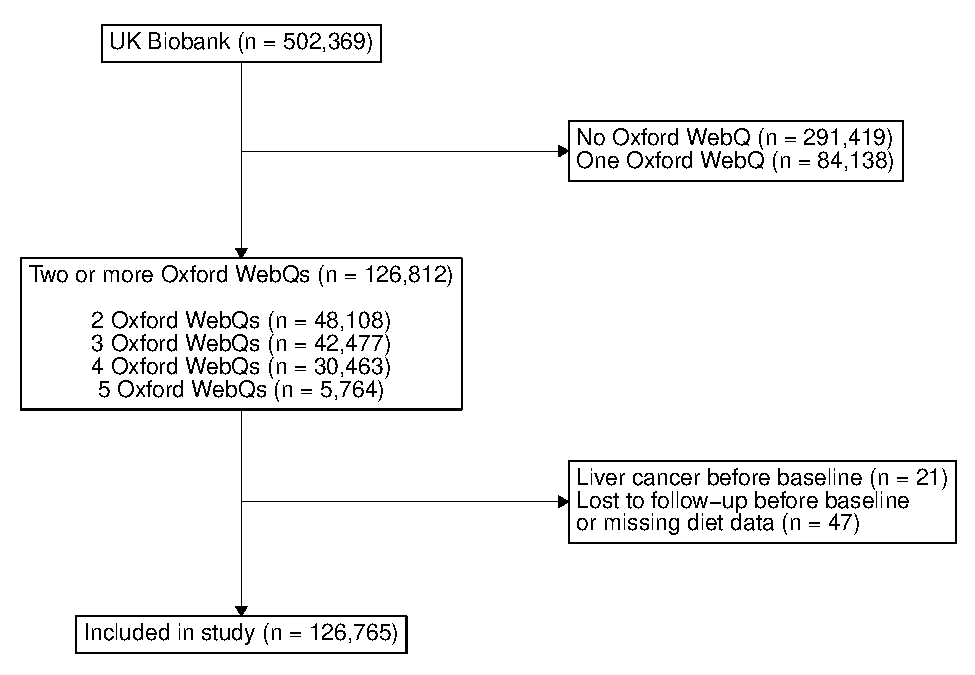
\includegraphics[width=0.75\linewidth,]{legliv_eur-j-nutr_files/figure-latex/fig1-1} 

}

\caption{Flowchart of included participants. Missing diet data were merged with loss to follow-up before baseline due to n being less than 5. It should be noted that not all UK Biobank participants were invited to complete an Oxfords WebQ. Only the last 70,000 participants to visit an assessment center were asked to complete an Oxford WebQ at the end of their visit. Further Oxford WebQs were sent to ~320,000 participants who provied an e-mail adress.}\label{fig:fig1}
\end{figure*}

During a median follow-up time of 11.3 years, 173 participants developed
liver cancer. Participants who developed liver cancer were older at
baseline, were more likely to be male, have a higher waist
circumference, be less physically active, and fewer had never smoked,
compared to all included participants (Table \ref{tab1}).

\begin{table*}
\caption{{\small \textbf{Baseline characteristics of UK Biobank participants who completed $\geq$ 2 Oxford WebQ 24-hour diet recall.}}}\label{tab1}
\begin{tabular*}{1\linewidth}{@{\extracolsep{\fill}}lcc}
\toprule
 & \textbf{Cohort} & \textbf{Liver cancer} \\ 
\cmidrule(lr){2-2} \cmidrule(lr){3-3}
\textbf{Variable} & \textbf{N = 126,744}\textsuperscript{\textit{1}} & \textbf{N = 173}\textsuperscript{\textit{1}} \\ 
\midrule\addlinespace[2.5pt]
{\bfseries Typical diet yesterday}\textsuperscript{\textit{2}} & 73,213 (58\%) & 105 (61\%) \\ 
{\bfseries Age, years} & 60 (53, 65) & 64.0 (60.0, 68.0) \\ 
{\bfseries Sex} &  &  \\ 
    Female & 70,659 (56\%) & 65 (38\%) \\ 
    Male & 56,085 (44\%) & 108 (62\%) \\ 
{\bfseries Educational level}\textsuperscript{\textit{3}} &  &  \\ 
    High & 59,416 (47\%) & 76 (44\%) \\ 
    Intermediate & 41,817 (33\%) & 52 (30\%) \\ 
    Low & 25,472 (20\%) & 45 (26\%) \\ 
    Missing & 39 &  \\ 
{\bfseries Townsend Deprivation Index} & -2.4 (-3.8, 0.0) & -2.6 (-3.7, -0.7) \\ 
    Missing & 149 &  \\ 
{\bfseries Living alone} & 22,658 (18\%) & 34 (20\%) \\ 
    Missing & 171 &  \\ 
{\bfseries Physical activity}\textsuperscript{\textit{4}} &  &  \\ 
    Above & 58,111 (46\%) & 61 (35\%) \\ 
    Below & 50,712 (40\%) & 79 (46\%) \\ 
    Missing & 17,921 (14\%) & 33 (19\%) \\ 
{\bfseries Smoking} &  &  \\ 
    Never & 72,583 (57\%) & 75 (43\%) \\ 
    Ever & 54,122 (43\%) & 98 (57\%) \\ 
    Missing & 39 &  \\ 
{\bfseries Alcohol intake, g/day} & 11 (0, 26) & 11 (0, 29) \\ 
{\bfseries Waist circumference, cm} & 88 (79, 97) & 98 (89, 107) \\ 
    Missing & 168 &  \\ 
\bottomrule
\end{tabular*}
\begin{minipage}{\linewidth}
\textsuperscript{\textit{1}}Median (IQR) for continous variables; n (\%) for categorical variables\\
\textsuperscript{\textit{2}}Participants who reported eating a typical diet yesterday for all completed diet questionnaires.\\
\textsuperscript{\textit{3}}High: College or University degree;
Intermediate: A levels/AS levels, O levels/GCSEs, or equivalent;
Low: none of the previous mentioned.\\
\textsuperscript{\textit{4}}Above or below the 2017 UK Physical activity guidelines of 150 minutes of moderate activity per week or 75 minutes of vigorous activity.\\
\end{minipage}
\end{table*}

Mean daily energy and total food intakes as well as daily intake of all
specified food groups in grams are presented in Table \ref{tab-diet}.

\begin{table*}
\caption{{\small \textbf{Daily dietary intake of food groups, total food and total energy intake in UK Biobank participants who completed $\geq$ 2 Oxford WebQ 24-hour diet recall.}}}\label{tab-diet}
\begin{tabular*}{1\linewidth}{@{\extracolsep{\fill}}lcc}
\toprule
 & \textbf{Cohort} & \textbf{Liver cancer} \\ 
\cmidrule(lr){2-2} \cmidrule(lr){3-3}
\textbf{Daily food intake} & \textbf{N = 126,744}\textsuperscript{\textit{1}} & \textbf{N = 173}\textsuperscript{\textit{1}} \\ 
\midrule\addlinespace[2.5pt]
\multicolumn{3}{l}{{\bfseries Total food intake}} \\ 
\midrule\addlinespace[2.5pt]
Energy, kJ & 8,430 (7,179, 9,856) & 8,579 (7,413, 10,048) \\ 
Weight, g & 3,144 (2,720, 3,621) & 3,162 (2,737, 3,659) \\ 
\midrule\addlinespace[2.5pt]
\multicolumn{3}{l}{{\bfseries Food groups, g/day}} \\ 
\midrule\addlinespace[2.5pt]
Legumes & 11 (0, 34) & 8 (0, 35) \\ 
Red and processed meat & 53 (15, 86) & 60 (30, 95) \\ 
Red meat & 30 (0, 60) & 45 (0, 73) \\ 
Processed meat & 9 (0, 30) & 8 (0, 31) \\ 
Other animal-based foods\textsuperscript{\textit{2}} & 475 (361, 603) & 448 (322, 604) \\ 
Healthy plant-based foods\textsuperscript{\textit{3}} & 1,806 (1,454, 2,198) & 1,791 (1,365, 2,158) \\ 
Unhealthy plant-based foods\textsuperscript{\textit{4}} & 472 (324, 662) & 491 (365, 698) \\ 
Alcoholic beverages & 132 (0, 342) & 144 (0, 375) \\ 
\bottomrule
\end{tabular*}
\begin{minipage}{\linewidth}
\textsuperscript{\textit{1}}Median (IQR)\\
\textsuperscript{\textit{2}}Other animal-based foods include: poultry, fish, dairy, eggs, and mixed dishes with animal products.\\
\textsuperscript{\textit{3}}Healthy plant-based foods include: whole grains, vegetables, fruits, nuts, plant oils, and beverages (coffee, tea, water).\\
\textsuperscript{\textit{4}}Unhealthy plant-based foods includes: refined grains, potatoes, mixed vegetarian dishes, sweets and snacks, fruit juice, and sugar sweetened beverages.\\
\end{minipage}
\end{table*}

No evidence of associations was found for substituting 15 g/day of
legumes with 15 g/day of total red meat, unprocessed red meat, or
processed red meat and risk of primary liver cancer in Model 1 (Table
\ref{tab-main}: total red meat:
HR: 0.98, 95\% CI: 0.93-1.04;
unprocessed red meat:
HR: 0.97, 95\% CI: 0.91-1.03;
processed red meat:
HR: 1.02, 95\% CI: 0.93-1.13).
The estimated associations changed minimally with further adjustments.
There was weak evidence of an association between replacement of
processed red meat with legumes (
HR: 1.09, 95\% CI: 0.98-1.20;
Table \ref{tab-main}).

\begin{table*}
\caption{{\small \textbf{Substitution of total meat, red meat and processed meat with legumes and hazard ratios and 95\% confidence intervals for primary liver cancer.}}}\label{tab-main}
\begin{tabular*}{1\linewidth}{@{\extracolsep{\fill}}lcc}
\toprule
 & {\bfseries \textbf{Model 1}}\textsuperscript{\textit{1}} & {\bfseries \textbf{Model 2}}\textsuperscript{\textit{2}} \\ 
\cmidrule(lr){2-2} \cmidrule(lr){3-3}
\textbf{15 g/day of legumes replacing:} & \textbf{HR} \textbf{(95\% CI)} & \textbf{HR} \textbf{(95\% CI)} \\ 
\midrule\addlinespace[2.5pt]
Total red meat & 0.98 (0.93-1.04) & 1.02 (0.96-1.08) \\ 
Unprocessed red meat & 0.97 (0.91-1.03) & 1.00 (0.94-1.07) \\ 
Processed red meat & 1.02 (0.93-1.13) & 1.09 (0.98-1.20) \\ 
\bottomrule
\end{tabular*}
\begin{minipage}{\linewidth}
\textsuperscript{\textit{1}}Adjusted for age (as underlying timescale), other food groups, and total food intake.\\
\textsuperscript{\textit{2}}Further adjusted for sex, educational level, Townsend deprivation index, living alone, physical activity, smoking, alcohol intake, and waist circumference.\\
\end{minipage}
\end{table*}

In secondary analyses, when analyzing the associations between
replacement of meat with legumes and HCC or ICC separately, weak
evidence of a higher risk of HCC was observed (Table \ref{tab-cancer},
total red meat:
HR: 1.06, 95\% CI: 0.97-1.16;
red meat:
HR: 1.05, 95\% CI: 0.96-1.15;
processed red meat:
HR: 1.09, 95\% CI: 0.95-1.26).
This was similar for ICC (Table \ref{tab-cancer}, total red meat:
HR: 0.97, 95\% CI: 0.90-1.05;
red meat:
HR: 0.95, 95\% CI: 0.87-1.03;
processed red meat:
HR: 1.07, 95\% CI: 0.93- 1.22).
The magnitude or direction of associations were not significantly
different across strata of liver cancer types.

In the adjusted non-substitution analysis, only the first quartile of
legume intake (mean intake 6.3 grams/day) was associated with a lower
risk of liver cancer, compared to no intake
(HR: 0.59, 95\% CI: 0.35-0.98);
no associations were observed for quartiles 2, 3 or 4 compared to no
intake (Table \ref{tab-legume}).

In sensitivity analyses, excluding participants based on high alcohol
intake, implau- sible energy intake, any liver disease or cancer before
baseline, or fewer than 3 completed Oxford WebQs did not alter the
estimates appreciably. Similar results were also found when including
death registries as a source of liver cancer cases and when excluding
waist circumference from the fully adjusted analysis (Supplementary
table \ref{tab-sens}).

\hypertarget{sec4}{%
\section{Discussion}\label{sec4}}

Contrary to our hypothesis, in this study we found little evidence of an
association between replacing 15g/day of red or processed meat with
legumes on risk of primary liver cancer. The estimates were robust to
our sensitivity analyses. When investigating liver cancer types
separately, replacing total red meat and unprocessed red meat with
legumes showed some weak evidence of an inverse association with ICC.
Our results for legume intake without specified substitutions did not
show a clear pattern of association.

This study had some limitations. First, none of the registries used to
determine a diagnosis of liver cancer were complete or up-to-date at the
time of analysis \citep{RN112}. Data from external providers, such as the NHS
England, NHS Central Register or National Records of Scotland, were
estimated to be mostly complete by the UK Biobank at various dates,
ranging from 31 December 2016 for cancer data from Wales to 31 October
2022 for hospital inpatient data from England \citep{RN114}. This could
introduce misclassification of the outcome, as individuals with liver
cancer may not be identified as cases. However, the estimates were
robust in a sensitivity analysis that included death registries as an
additional source of liver cancer diagnoses to accommodate missing
outcome events. Incorrectly classifying non-cases as cases would lead to
attenuation of our results, but this is unlikely due to register
linkage. Second, the relatively low number of events limited our ability
to adjust for confounding factors. Excessive adjustment parameters per
event can compromise the validity of the multivariable Cox regression
model, potentially causing biased estimates. To ensure statistical
validity, we aimed for at least 10 events per variable in the main
analysis by limiting the number of adjustment levels, using fewer and
broader food groups, and fewer levels for categorical covariates. This
approach was guided by our \emph{a priori} causal assumptions. Although this
method helped maintain statistical validity, it may have increased
residual confounding by diluting the importance of specific food groups.
Additionally, risk factors that we could not adjust for, such as
aflatoxin B1, a known liver carcinogen, may have contributed to residual
confounding. Third, by specifying that the dietary exposure was
collected on at least two occasions, our study population suffered
considerable attrition. This is unlikely to be completely at random, and
most likely resulted in a study population with greater focus on their
dietary habits. For example, the mean intake of processed meat was low
in our study population. If a diet consisting of higher intakes of
healthier plant-based foods is associated with lower liver cancer
incidence, our study population may be at lower risk overall, thus
reducing the power of our study to detect an association.

Strengths of this study are the prospective longitudinal design, which
establish temporality between the diet exposure and liver cancer
outcome, and the large sample size, which enabled analyses of a rare
cancer. Though health registries may have been only partially up to
date, using registries almost eliminates selection bias due to loss to
follow-up. Estimates were robust to exclusion of participants with fewer
than three completed Oxford WebQs, indicating that at least two 24-hour
diet recall measurements were sufficient to estimate diet over time.
Further, our specified substitution analyses have some strengths in
contrast to traditional methods in nutritional epidemiology through
examining the effect of consuming a food or nutrient while holding all
other foods constant. The substitution is easily interpretable and
reflects the implications that an increased intake of a food is at the
expense a decreased intake of other foods. In that sense, the food
substitution model mimics some aspects of a randomized controlled
design.

Contrary to our hypothesis, replacing processed red meat with legumes
was associated with a non-significant increase in risk of primary liver
cancer, with a greater effect size compared to unprocessed red meat.
This pattern persisted across all sensitivity analyses. However, the
estimates for processed red meat were labeled with less confidence,
partly due to the low median intake. These findings align with recent
analyses from the UK Biobank, which indicated that unprocessed red meat
intake was associated with a non-significant increase in liver cancer
risk, with a greater effect size than processed meat (both white and red
meat) \citep{Knuppel2020}. This supports the notion that processed meat may
not be associated with liver cancer risk in this population.

The literature on food substitutions, particularly in relation to liver
cancer, is sparse. Accordingly, we also conducted an analysis of legume
intake without specifying food substitutions. However, a recent
meta-anlysis of observational studies found a non-linear dose-response
relationship between legume intake and liver cancer risk, with a
protective effect observed between intakes of 8 g/day to 40 g/day
\citep{liu2023a}. This somewhat contrasts with our findings where any
increase above 6.3 g/day of legumes was not associated with a decreased
risk of liver cancer, compared to no legume intake. A recent
meta-analysis of observational studies showed no association between red
or processed meat intake and HCC \citep{Di2023}.

\hypertarget{sec5}{%
\section{Conclusion}\label{sec5}}

Supplementary table \ref{tab-sens}

\begin{appendices}

\renewcommand{\thetable}{S\arabic{table}} \renewcommand{\theHtable}{S\arabic{table}}
\renewcommand{\thefigure}{S\arabic{figure}} \renewcommand{\theHfigure}{S\arabic{figure}}

\clearpage

\hypertarget{secA1}{%
\section{Supplementary material}\label{secA1}}

\begin{figure*}[h]

{\centering 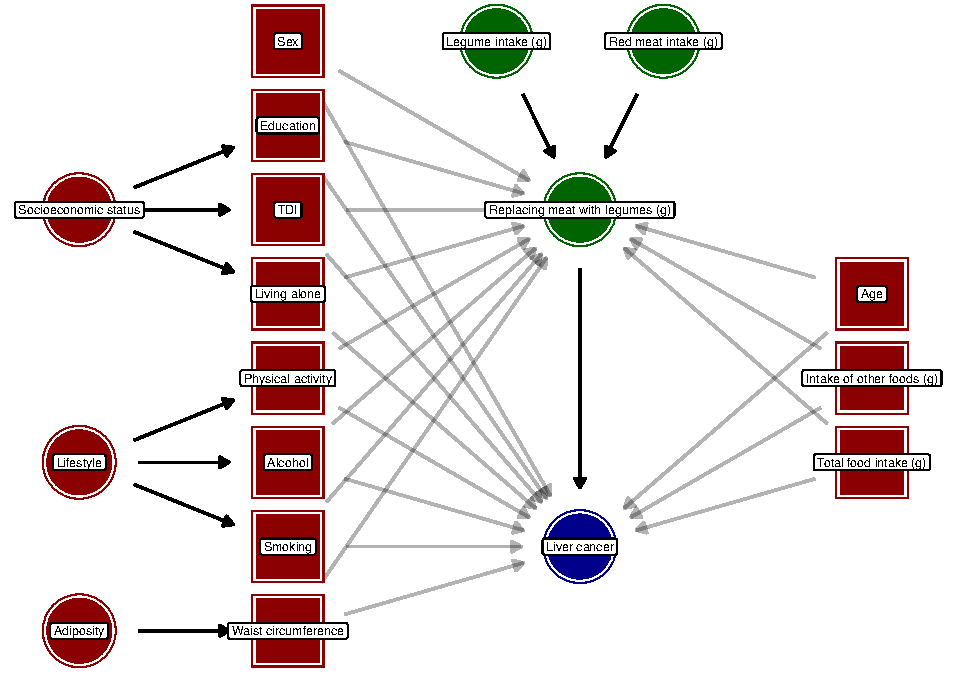
\includegraphics[width=1\linewidth,]{legliv_eur-j-nutr_files/figure-latex/fig2-1} 

}

\caption{Simplified directed acyclic graph (DAG) visualizing the hypothesised causal relationship between replacing red meat with legumes and liver cancer based on assumptions of biasing paths. Red nodes represent confounders. Square nodes represent the minimal sufficient adjustment set for estimating the effect of replacing red meat with legumes on liver cancer. Shadowed arrows represent biasing paths. DAG terminology demands visualisation of all hypothesized correlating relationships between variables, typically resulting in complex an hard-to-follow illustrations. To improve readability, inter-covariate arrows are hidden in the above DAG.}\label{fig:fig2}
\end{figure*}

\clearpage

\begin{table*}[!t]
\caption{{\small \textbf{Summary of included foods for each food group.}}}\label{tab-food-group}
\begin{tabular*}{1\linewidth}{@{\extracolsep{\fill}}>{\raggedright\arraybackslash}p{\dimexpr 0.2\linewidth-2\tabcolsep-1.5\arrayrulewidth}>{\raggedright\arraybackslash}p{\dimexpr 0.8\linewidth-2\tabcolsep-1.5\arrayrulewidth}}
\toprule
\textbf{Food group} & \textbf{Includes} \\ 
\midrule\addlinespace[2.5pt]
{\bfseries Legumes} & Soya-based desserts, Baked beans, pulses, Soya drinks (including calcium fortified),
  Tofu-based products, Hummus, Peas \\ 
{\bfseries Red meat} & Beef, Lamb, Other meat including offal, Pork \\ 
{\bfseries Processed meat} & Sausages, bacon (with and without fat), ham, liver pate \\ 
{\bfseries Animal-based foods} & Poultry, fish, dairy, eggs, mixed dishes, and sauces and condiments \\ 
{\bfseries Healthy plant-based foods} & Whole grains, fruits, nuts, plant oils, beverages (water, tea and coffee), vegetables \\ 
{\bfseries Unhealthy plant-based foods} & Refined cereals, potatoes, fruit juice, mixed dishes (vegetarian), sweets \& snacks, and sugar sweetened beverages \\ 
{\bfseries Alcoholic beverages} & Beer and cider, spirits and other alcoholic drinks, fortified wine, red and rose wine, white wine \\ 
\bottomrule
\end{tabular*}
\end{table*}

\begin{table*}[!t]
\caption{{\small \textbf{Substitution of total meat, red meat and processed meat with legumes and hazard ratios and 95\% confidence intervals for hepatocellular carcinoma and intrahepatic cholangiocarcinoma.}}}\label{tab-cancer}
\begin{tabular*}{1\linewidth}{@{\extracolsep{\fill}}lcc}
\toprule
 & \textbf{Model 1}\textsuperscript{\textit{1}} & \textbf{Model 2}\textsuperscript{\textit{2}} \\ 
\cmidrule(lr){2-2} \cmidrule(lr){3-3}
\textbf{15 g/day of legumes replacing:} & \textbf{HR} \textbf{(95\% CI)} & \textbf{HR} \textbf{(95\% CI)} \\ 
\midrule\addlinespace[2.5pt]
\multicolumn{3}{l}{{\bfseries Hepatocellular carcinoma}} \\ 
\midrule\addlinespace[2.5pt]
Total red meat & 1.01 (0.93-1.10) & 1.06 (0.97-1.16) \\ 
Unprocessed red meat & 1.01 (0.92-1.11) & 1.05 (0.96-1.15) \\ 
Processed red meat & 1.01 (0.88-1.16) & 1.09 (0.95-1.26) \\ 
\midrule\addlinespace[2.5pt]
\multicolumn{3}{l}{{\bfseries Intrahepatic cholangiocarcinoma}} \\ 
\midrule\addlinespace[2.5pt]
Total red meat & 0.94 (0.87-1.02) & 0.97 (0.90-1.05) \\ 
Unprocessed red meat & 0.92 (0.85-1.00) & 0.95 (0.87-1.03) \\ 
Processed red meat & 1.02 (0.89-1.17) & 1.07 (0.93-1.22) \\ 
\bottomrule
\end{tabular*}
\begin{minipage}{\linewidth}
\textsuperscript{\textit{1}}Adjusted for age (as underlying timescale), other food groups, and total food intake.\\
\textsuperscript{\textit{2}}Further adjusted for sex, educational level, Townsend deprivation index, living alone, physical activity, smoking, alcohol intake, and waist circumference.\\
\end{minipage}
\end{table*}

\begin{table*}[!t]
\caption{{\small \textbf{No intake of legumes vs. quartiles of daily legume intake and hazard ratios and 95\% confidence intervals for primary liver cancer.}}}\label{tab-legume}
\begin{tabular*}{1\linewidth}{@{\extracolsep{\fill}}lccc}
\toprule
 &  & \textbf{Model 1}\textsuperscript{\textit{1}} & \textbf{Model 2}\textsuperscript{\textit{2}} \\ 
\cmidrule(lr){3-3} \cmidrule(lr){4-4}
\textbf{Characteristic} & \textbf{Mean daily legume intake} & \textbf{HR} \textbf{(95\% CI)} & \textbf{HR} \textbf{(95\% CI)} \\ 
\midrule\addlinespace[2.5pt]
Categories: &  &  &  \\ 
    No intake & 0.00 & — & — \\ 
    Q1 & 6.3 & 0.58 (0.35-0.96) & 0.59 (0.35-0.98) \\ 
    Q2 & 16 & 0.87 (0.56-1.33) & 0.89 (0.58-1.36) \\ 
    Q3 & 34 & 0.75 (0.47-1.19) & 0.75 (0.47-1.19) \\ 
    Q4 & 109 & 0.98 (0.64-1.51) & 1.06 (0.69-1.64) \\ 
\bottomrule
\end{tabular*}
\begin{minipage}{\linewidth}
\textsuperscript{\textit{1}}Adjusted for age (as underlying timescale), other food groups, and total food intake.\\
\textsuperscript{\textit{2}}Further adjusted for sex, educational level, Townsend deprivation index, living alone, physical activity, smoking, alcohol intake, and waist circumference.\\
\end{minipage}
\end{table*}

\begin{sidewaystable*}[!t]
\caption{{\small \textbf{Sensitivity analyses}}}\label{tab-sens}
\fontsize{7.5pt}{9.0pt}\selectfont
\begin{tabular*}{1\linewidth}{@{\extracolsep{\fill}}>{\raggedright\arraybackslash}p{\dimexpr 0.125\linewidth-2\tabcolsep-1.5\arrayrulewidth}>{\centering\arraybackslash}p{\dimexpr 0.125\linewidth-2\tabcolsep-1.5\arrayrulewidth}>{\centering\arraybackslash}p{\dimexpr 0.125\linewidth-2\tabcolsep-1.5\arrayrulewidth}>{\centering\arraybackslash}p{\dimexpr 0.125\linewidth-2\tabcolsep-1.5\arrayrulewidth}>{\centering\arraybackslash}p{\dimexpr 0.125\linewidth-2\tabcolsep-1.5\arrayrulewidth}>{\centering\arraybackslash}p{\dimexpr 0.125\linewidth-2\tabcolsep-1.5\arrayrulewidth}>{\centering\arraybackslash}p{\dimexpr 0.125\linewidth-2\tabcolsep-1.5\arrayrulewidth}>{\centering\arraybackslash}p{\dimexpr 0.125\linewidth-2\tabcolsep-1.5\arrayrulewidth}}
\toprule
 & \multicolumn{5}{c}{\textbf{Exclusion of participants with:}} &  &  \\ 
\cmidrule(lr){2-6}
 & \textbf{High alcohol intake}\textsuperscript{\textit{1}} & \textbf{Implausible food intake}\textsuperscript{\textit{2}} & \textbf{Liver disease before baseline}\textsuperscript{\textit{3}} & \textbf{Any cancer before baseline}\textsuperscript{\textit{4}} & \textbf{Fewer than 3 Oxford WebQs} & \textbf{Death register as source of liver cancer events} & \textbf{Exclusion of waist circumference from analysis} \\ 
\cmidrule(lr){2-2} \cmidrule(lr){3-3} \cmidrule(lr){4-4} \cmidrule(lr){5-5} \cmidrule(lr){6-6} \cmidrule(lr){7-7} \cmidrule(lr){8-8}
\textbf{15 g/day of legumes replacing:} & \textbf{HR} \textbf{(95\% CI)} & \textbf{HR} \textbf{(95\% CI)} & \textbf{HR} \textbf{(95\% CI)} & \textbf{HR} \textbf{(95\% CI)} & \textbf{HR} \textbf{(95\% CI)} & \textbf{HR} \textbf{(95\% CI)} & \textbf{HR} \textbf{(95\% CI)} \\ 
\midrule\addlinespace[2.5pt]
Total red meat & 1.00 (0.94-1.07) & 1.01 (0.94-1.08) & 0.99 (0.93-1.06) & 1.04 (0.97-1.11) & 1.04 (0.97-1.12) & 1.02 (0.97-1.09) & 1.00 (0.94-1.06) \\ 
Unprocessed red meat & 0.99 (0.92-1.05) & 0.98 (0.91-1.06) & 0.97 (0.91-1.04) & 1.01 (0.94-1.09) & 1.02 (0.94-1.11) & 1.01 (0.95-1.07) & 0.99 (0.92-1.05) \\ 
Processed red meat & 1.06 (0.95-1.17) & 1.10 (0.98-1.24) & 1.07 (0.96-1.20) & 1.15 (1.01-1.30) & 1.11 (0.97-1.27) & 1.07 (0.97-1.18) & 1.05 (0.95-1.16) \\ 
\bottomrule
\end{tabular*}
\begin{minipage}{\linewidth}
\textsuperscript{\textit{1}}Exclusion of the upper decile of alcohol intake (g/day) for each sex.\\
\textsuperscript{\textit{2}}Exclusion of the upper and lower decile of energy intake (kJ/day) for each sex.\\
\textsuperscript{\textit{3}}ICD10 codes: K70-79, B16-19, Z94.4, I82.0, I85, I86.4, E83.0-1 and E88. ICD9 codes: 571-574, 070, V427 and 2750-2751.\\
\textsuperscript{\textit{4}}ICD10 codes: C00-C97 and D00-D48. ICD9 codes: 140-239.\\
\end{minipage}
\end{sidewaystable*}

\begin{verbatim}
## \begin{table*}[!t]
## \caption{{\small \textbf{Substitution of total meat, red meat and processed meat with legumes and hazard ratios and 95\% confidence intervals for hepatocellular carcinoma and intrahepatic cholangiocarcinoma.}}}\label{tab:tab-cancer}
## \begin{tabular*}{1\linewidth}{@{\extracolsep{\fill}}lcc}
## \toprule
##  & \textbf{Model 1}\textsuperscript{\textit{1}} & \textbf{Model 2}\textsuperscript{\textit{2}} \\
## \cmidrule(lr){2-2} \cmidrule(lr){3-3}
## \textbf{15 g/day of legumes replacing:} & \textbf{HR} \textbf{(95\% CI)} & \textbf{HR} \textbf{(95\% CI)} \\
## \midrule\addlinespace[2.5pt]
## \multicolumn{3}{l}{{\bfseries Hepatocellular carcinoma}} \\
## \midrule\addlinespace[2.5pt]
## Total red meat & 1.01 (0.93-1.10) & 1.06 (0.97-1.16) \\
## Unprocessed red meat & 1.01 (0.92-1.11) & 1.05 (0.96-1.15) \\
## Processed red meat & 1.01 (0.88-1.16) & 1.09 (0.95-1.26) \\
## \midrule\addlinespace[2.5pt]
## \multicolumn{3}{l}{{\bfseries Intrahepatic cholangiocarcinoma}} \\
## \midrule\addlinespace[2.5pt]
## Total red meat & 0.94 (0.87-1.02) & 0.97 (0.90-1.05) \\
## Unprocessed red meat & 0.92 (0.85-1.00) & 0.95 (0.87-1.03) \\
## Processed red meat & 1.02 (0.89-1.17) & 1.07 (0.93-1.22) \\
## \bottomrule
## \end{tabular*}
## \begin{minipage}{\linewidth}
## \textsuperscript{\textit{1}}Adjusted for age (as underlying timescale), other food groups, and total food intake.\\
## \textsuperscript{\textit{2}}Further adjusted for sex, educational level, Townsend deprivation index, living alone, physical activity, smoking, alcohol intake, and waist circumference.\\
## \end{minipage}
## \end{table*}
\end{verbatim}

\end{appendices}

\clearpage

\bibliography{bibliography.bib}


\end{document}
